\documentclass[preprint,12pt,authoryear]{elsarticle}

\usepackage{amsmath,amssymb}
\usepackage{booktabs}
\usepackage{graphicx}
\usepackage{multirow}
\usepackage{xcolor}
\usepackage{url}
\usepackage{placeins}
\setlength{\emergencystretch}{3em}

\journal{Computers and Electronics in Agriculture}

\newcommand{\model}{PhytoODE}
\newcommand{\todo}[1]{#1}

\begin{document}

\begin{frontmatter}

\title{PhytoODE: Learning plant growth dynamics across genotypes, temperature, and light regimes}

\author[inst1]{Yeoul Lim}
\author[inst1]{Siyoung You}
\author[inst2]{Hanim Kim}
\author[inst1]{Hwijae Son}

\address[inst1]{\todo{Department of Mathematics, Konkuk University, Seoul, Republic of Korea}}
\address[inst2]{\todo{Department of Chemistry, Seoul National University, Seoul, Republic of Korea}}

\begin{abstract}
Predicting plant growth across genotypes and environments requires flexible dynamics under sparse observation. We present \model{}, a genotype- and environment-conditioned latent neural ordinary differential equation model. An encoder reads a known environmental scenario, a learned latent flow evolves continuously, and a decoder predicts phenotype without target-curve measurements as inputs. Logistic derivative and capacity penalties weakly regularize the decoded trajectory. Three temperature-conditioned benchmarks cover wheat with 19 genotypes, UAV maize with 402 genotypes, and Arabidopsis stem length with four observations per plant. Mean test RMSEs were $0.03032$~m, $56.68$ relative UAV-height units, and $2.800$~cm, respectively, corresponding to relative RMSEs of $10.24\%$, $18.40\%$, and $14.06\%$. These were lower than the compared benchmark families and matched no-physics controls. A fourth, author-collected dataset comprises 1,818 hypocotyl measurements across five genotypes and two light regimes at 23~$^{\circ}$C. A light-switched logistic constraint introduces separate effective light and dark growth rates. In this experiment, all models learn directly from individual measured lengths, with no phenotype imputation or replicate averaging. On 436 held-out measurements, \model{} achieved $0.779$~mm RMSE ($13.72\%$ relative RMSE); the independently tuned no-physics latent ODE obtained $0.782$~mm ($13.77\%$). The experiments address field-season transfer, genotype-panel scale, sparse temporal sampling, and environmental-driver substitution. Evaluated genotypes and treatment regimes are represented during training.
\end{abstract}

\begin{keyword}
plant growth \sep plant height \sep latent neural ODE \sep physics-informed learning \sep genotype--environment interaction \sep sparse time series \sep Arabidopsis thaliana \sep wheat \sep maize \sep UAV phenotyping
\end{keyword}

\end{frontmatter}


\section{Introduction}
\label{sec:introduction}

Repeated phenotyping has shifted crop modelling from end-point prediction toward the analysis of complete growth trajectories. High-resolution imaging and sensor systems now quantify crop traits across space and time \citep{zhang2020phenotyping,kim2023monitoring,ehret2011tomato}, while time-series remote sensing and image-generation methods have enabled crop mapping and visual growth forecasting \citep{wang2021sentinel,drees2021brassica}. These measurements are valuable because plant growth is a dynamic response to genotype, development, and changing environmental conditions rather than a static trait. Nevertheless, longitudinal measurements remain expensive and irregular in many experiments, and measurements from different studies can range from daily field trajectories to only a few destructive or manual observations.

Machine learning has been applied widely to weather-conditioned crop prediction. Examples include wheat and maize yield forecasting from vegetation-index time series \citep{nagy2018forecasting}, farm-level and durum-wheat prediction \citep{tesfaye2021wheat,chergui2022durum}, hybrid performance prediction in corn \citep{sarijaloo2021corn}, and stacked recurrent models that combine unmanned-aerial-vehicle and meteorological time series \citep{wang2025sugarbeet}. Related studies have learned crop responses to temperature or limited climate information \citep{sharma2022evapotranspiration,singh2023eto}, grapevine phenology from climate records \citep{fasihi2025phenology}, and crop stress from biological signals \citep{wen2025stress}. Deep networks can also identify critical weather windows for spring wheat \citep{benke2025weather}, but purely data-driven models may require substantial data and can learn statistical shortcuts that are difficult to reconcile with biological growth.

Genotype--environment interaction further complicates temporal prediction. Multi-environment analyses must cope with incomplete genotype-by-environment matrices \citep{arciniegas2020imputation}, nonlinear interactions \citep{patil2023genotype}, and environmentally dependent genetic performance \citep{li2026plasticity}. The challenge is not limited to yield: greenhouse regulation, water use, morphology, and fresh biomass couple plant state to environmental forcing at multiple scales \citep{gao2024ipecm,salagovic2025tomato,zhang2026lettuce}. Consequently, a useful trajectory model should share information across genotypes while preserving genotype-specific responses and should incorporate environmental drivers without requiring an independent model for every genotype.

Hybrid mechanistic--machine-learning approaches offer one route to this goal. Process-model simulations have been assimilated with hyperspectral observations \citep{wang2025gecros}, combined with remote sensing and machine learning for wheat prediction \citep{kheir2025hybrid}, and synthesized with deep learning to estimate wheat biomass dynamics \citep{chen2026biomass}. Hybridization is especially appealing when training datasets are small \citep{dhal2022aquaponic}, when model parsimony matters \citep{saravi2021variable}, or when explanations are required \citep{ryo2022xai,ennaji2023nutrient}. Reservoir and pretrained sequence models provide additional options for vegetation-index forecasting \citep{olamofe2025ndvi}. Most directly, \citet{shao2026pinn} combined a logistic growth equation with an LSTM in a physics-informed neural network (Logi-PINN) for wheat plant-height prediction. Their results demonstrated the promise of weak biological constraints, but the observed height remained tied to a predetermined scalar logistic law whose adequacy can vary across genotype, environment, organ, and species.

Neural ordinary differential equations replace discrete hidden-state transitions with a learned continuous vector field \citep{chen2018neuralode}. Latent ODEs extend this idea by evolving an unobserved state that can represent richer dynamics than a single measured variable and are naturally compatible with irregular observation times \citep{rubanova2019latentode}. Augmenting the latent state can increase expressiveness and improve numerical behaviour \citep{dupont2019augmented}, while neural controlled differential equations formalize continuous-time responses to incoming covariates \citep{kidger2020neuralcde}. These ideas are complementary to physics-informed learning \citep{raissi2019pinn,karniadakis2021piml} and universal differential equations, which combine known and learned dynamics \citep{rackauckas2020ude}. Despite this methodological fit, latent continuous-time models have not been adequately tested for genotype-conditioned plant growth across both field-scale dense trajectories and extremely sparse external biological datasets.

We introduce \model{}, a latent neural ODE model that shares parameters across genotypes and learns environment-conditioned growth dynamics. A weak logistic residual is retained as a regularizer rather than imposed as the complete state equation. We make five contributions: (i) a continuous-time architecture that predicts an entire genotype-specific growth curve from genotype, time, and a known environmental scenario, without using phenotype observations from the target trajectory; (ii) a protocol-matched, year-held-out wheat evaluation aligned with \citet{shao2026pinn}; (iii) a year-held-out UAV maize evaluation spanning 402 genotypes, which tests whether a learned genotype-conditioned dynamical system remains effective at substantially greater genetic scale; (iv) an external \textit{Arabidopsis thaliana} stem-length evaluation with only four observations per plant; and (v) an author-collected hypocotyl experiment under two light regimes at fixed temperature, with held-out replicate measurements and a reproducible dataset package. Together, the datasets vary in species, organ, physical scale, genotype count, temporal resolution, and generalization unit.


\section{Materials and methods}
\label{sec:methods}

\subsection{Prediction task}

Let $g\in\{1,\ldots,G\}$ denote genotype, $\mathbf u_g(t)$ a known environmental scenario, and $y_g(t_i)$ the observed growth phenotype at a subset of times $\mathcal{O}_g$. The environmental input is temperature in the first three datasets and illumination plus duty cycle in the hypocotyl experiment. The model predicts a complete trajectory $\hat y_g(t)$ on a common integration grid. Missing phenotype times do not contribute to the data loss. The principal task is trajectory-level generalization: to a held-out year for wheat and maize and to new biological replicate plants for Arabidopsis stem length. The hypocotyl experiment evaluates held-out replicate measurements at the same observed times. In all four datasets, the evaluated genotype labels are present during training.

This implementation is an offline, scenario-conditioned predictor. The environmental scenario over the prediction interval is assumed known and is read by the initial-state encoder. No phenotype observation from an evaluated curve is used as an input. A causal real-time forecast would require restricting the encoder to information available at the forecast origin.

\subsection{\model{} architecture: genotype- and environment-conditioned latent dynamics}

Each genotype is represented by a $d_e$-dimensional embedding $\mathbf e_g$ learned from a one-hot vector. An LSTM encoder reads the environmental channels and normalized time in reverse temporal order and produces the initial latent state,
\begin{equation}
 \mathbf z_g(0)=E_{\phi}\!\left(\{\mathbf u_g(\tau_j),\tau_j\}_{j=1}^{J},\mathbf e_g\right),
 \qquad \mathbf z_g(0)\in\mathbb R^{d_z}.
 \label{eq:encoder}
\end{equation}
The latent state evolves according to
\begin{equation}
 \frac{d\mathbf z_g}{d\tau}
 =3\tanh\!\left[f_{\theta}\!\left(\mathbf z_g(\tau),\mathbf u_g(\tau),\mathbf e_g,\tau\right)\right],
 \qquad \tau\in[0,1],
 \label{eq:ode}
\end{equation}
where $f_{\theta}$ is a hyperbolic-tangent multilayer perceptron (MLP). For temperature-conditioned experiments, standardized temperature at intermediate solver stages is obtained by linear interpolation, and a fixed-step fourth-order Runge--Kutta solver uses one substep per daily interval. Discontinuous illumination uses a 3-h grid and piecewise-constant forcing, as detailed in Section~\ref{subsec:lightmodel}. Finally, an MLP decoder maps the latent trajectory to the phenotype,
\begin{equation}
 \hat y_g(\tau)=\operatorname{LeakyReLU}_{0.01}\!\left[D_{\psi}(\mathbf z_g(\tau))\right].
 \label{eq:decoder}
\end{equation}
For wheat, validation-only capacity tuning selected a 16-dimensional latent state, four-dimensional genotype embedding, one ODE hidden layer of width 16, decoder width 16, and LSTM encoder width 8, for 1,655 trainable parameters. The maize search selected latent dimension 8, genotype embedding 8, one ODE hidden layer of width 16, decoder width 32, and encoder width 32, for 9,003 parameters. Arabidopsis used the pre-tuning full-capacity instance: latent dimension 16, genotype embedding 4, two ODE hidden layers of width 32, decoder width 32, and encoder width 16, for 4,607 parameters. All experiments use the same continuous-time model family; capacity was selected separately where a validation search was conducted.

\subsection{Observable-space logistic regularization and derivative computation}

The latent vector field is learned freely, while the decoded phenotype is weakly encouraged to have a genotype-specific logistic growth rate. For clarity, let
\begin{equation}
 G_{\psi}(\mathbf z)
 =\operatorname{LeakyReLU}_{0.01}\!\left[D_{\psi}(\mathbf z)\right]
\end{equation}
denote the complete scalar decoder in Eq.~\eqref{eq:decoder}, including its output activation, and let $\mathbf F_{\theta}$ denote the right-hand side of Eq.~\eqref{eq:ode}. The decoder has no explicit time input, so its dependence on time is entirely through the latent trajectory. For trajectory $n$, belonging to genotype $g(n)$, we therefore have
\begin{equation}
 \hat y_n(\tau)=G_{\psi}\!\left(\mathbf z_n(\tau)\right),
 \qquad
 \frac{d\hat y_n}{d\tau}
 =\nabla_{\mathbf z}G_{\psi}\!\left(\mathbf z_n(\tau)\right)^{\!\top}
 \mathbf F_{\theta}\!\left(\mathbf z_n(\tau),\mathbf u_n(\tau),
 \mathbf e_{g(n)},\tau\right).
 \label{eq:decoder_chain_tau}
\end{equation}
Equation~\eqref{eq:decoder_chain_tau} is the directional derivative of the decoder along the learned latent flow. It does not assume that any individual latent coordinate represents height or follows logistic dynamics.

The ODE is solved on normalized time $\tau\in[0,1]$, whereas the reference growth rate uses physical time (days for the first three datasets and hours for hypocotyls). If $t=t_0+S\tau$, where $S=t_{\mathrm{last}}-t_0$ is the physical duration of the integration interval, a second application of the chain rule gives
\begin{equation}
 \frac{d\hat y_n}{dt}
 =\frac{1}{S}\frac{d\hat y_n}{d\tau}
 =\frac{1}{S}
 \nabla_{\mathbf z}G_{\psi}\!\left(\mathbf z_n(\tau)\right)^{\!\top}
 \mathbf F_{\theta}\!\left(\mathbf z_n(\tau),\mathbf u_n(\tau),
 \mathbf e_{g(n)},\tau\right).
 \label{eq:decoder_chain_day}
\end{equation}
The values of $S$ were 169, 95, and 22 days for wheat, maize, and Arabidopsis stem length, respectively, and 72 hours for hypocotyl length. This conversion is necessary because a derivative with respect to normalized time would otherwise change merely when the length of the study interval changed.

The derivative in Eq.~\eqref{eq:decoder_chain_day} is evaluated by automatic differentiation rather than by finite differences of predicted or observed heights. At each collocation node $(n,j)$, the vector field is re-evaluated at the stored latent state to obtain $\mathbf F_{\theta}(\mathbf z_{nj},\mathbf u_{nj},\mathbf e_{g(n)},\tau_j)$. In the same forward computation, reverse-mode automatic differentiation evaluates the decoder gradient $\nabla_{\mathbf z}G_{\psi}(\mathbf z_{nj})$. Operationally, the implementation forms
\begin{equation}
 Q=\sum_{n=1}^{N}\sum_{j=1}^{J}G_{\psi}(\mathbf z_{nj}),
 \qquad
 \frac{\partial Q}{\partial\mathbf z_{nj}}
 =\nabla_{\mathbf z}G_{\psi}(\mathbf z_{nj}),
 \label{eq:autodiff_decoder}
\end{equation}
where the equality follows because the decoder is applied independently to each trajectory--time pair. The elementwise inner product of this gradient and the vector field gives $d\hat y_n/d\tau$, which is divided by $S$ to obtain $d\hat y_n/dt$. Thus, no derivative target is estimated from sparse, irregular, or noisy phenotype measurements, and no finite-difference interval has to be chosen. The LeakyReLU decoder is piecewise differentiable, so the same operation differentiates the entire decoder, including the output activation.

The derivative computation is retained in the training computation graph. In particular, the automatic-differentiation call is made with graph construction enabled, and the fixed-step Runge--Kutta operations are not detached. Back-propagating the final objective can therefore update the decoder, the neural vector field, the initial-state environmental encoder, and the genotype embedding through the derivative residual. It also updates the genotype-specific logistic parameter head described below. This is what allows a loss defined on $d\hat y/dt$ to train the original model parameters even though height derivatives are never provided as observations.

For the temperature-conditioned datasets, a small MLP maps each genotype embedding to two constrained logistic parameters,
\begin{equation}
 r_g=\sigma(a_g), \qquad K_g=1+\tanh(b_g),
 \label{eq:logistic_parameters}
\end{equation}
where $r_g\in(0,1)$ day$^{-1}$ and $K_g\in(0,2)$ in the units used to train the phenotype output. Those units are metres for wheat and Arabidopsis and training-scaled relative-height units for maize; maize predictions are multiplied by the training-set scale factor for reporting. The pointwise logistic residual is
\begin{equation}
 \varepsilon_{nj}
 =\frac{d\hat y_n(t_j)}{dt}
 -r_{g(n)}\hat y_n(t_j)
 \left(1-\frac{\hat y_n(t_j)}{K_{g(n)}}\right),
\end{equation}
and the corresponding physics loss is
\begin{equation}
 \mathcal L_{\mathrm{phys}}
 =\frac{1}{N J}\sum_{n=1}^{N}\sum_{j=1}^{J}\varepsilon_{nj}^{2}.
 \label{eq:physics}
\end{equation}
In the temperature-conditioned experiments, the $J$ integration nodes act as deterministic collocation points. Consequently, Eq.~\eqref{eq:physics} is evaluated at every daily grid point of every training trajectory, including days at which phenotype is unobserved. It is not evaluated at the intermediate stage states used inside the Runge--Kutta update, and validation and test targets never enter this loss. In the sparse Arabidopsis setting, for example, four measured stem lengths determine the data term, but the physics term can still regularize the predicted daily trajectory over the full 23-day grid. These unobserved-grid residuals add a growth-shape prior rather than additional phenotype information.

Unlike a logistic ODE baseline, Eq.~\eqref{eq:physics} does not generate the trajectory and is not imposed as a hard equality. The learned, environment-conditioned latent vector field remains the trajectory-generating model, and the residual only penalizes disagreement between its decoded instantaneous growth rate and a logistic reference rate. The model can therefore depart from logistic behaviour when this improves agreement with the observed trajectories.

For the three temperature-conditioned datasets, the observed-data term is the mean of the per-trajectory masked RMSE,
\begin{equation}
 \mathcal L_{\mathrm{data}}
 =\frac{1}{N}\sum_{n=1}^{N}
 \sqrt{\frac{\sum_j m_{nj}(\hat y_{nj}-y_{nj})^2}
 {\sum_j m_{nj}}},
 \label{eq:data_loss}
\end{equation}
and the full objective is
\begin{equation}
 \mathcal L=\mathcal L_{\mathrm{data}}
 +\lambda_{\mathrm{phys}}\mathcal L_{\mathrm{phys}}
 +\lambda_K\mathcal L_K,
 \label{eq:loss}
\end{equation}
where
\begin{equation}
 \mathcal L_K
 =\frac{1}{N}\sum_{n=1}^{N}
 \left|\max_j\hat y_{nj}-K_{g(n)}\right|
\end{equation}
ties the genotype-specific carrying capacity to the largest predicted phenotype on each training trajectory. The distinction between the two principal terms is important: $\mathcal L_{\mathrm{data}}$ uses only positions selected by the observation mask $m_{nj}$, whereas $\mathcal L_{\mathrm{phys}}$ and $\mathcal L_K$ use the complete predicted grid. We denote the coefficient of the ODE derivative residual by $\lambda_{\mathrm{ODE}}\equiv\lambda_{\mathrm{phys}}$. The reported $(\lambda_{\mathrm{ODE}},\lambda_K)$ pairs are $(3.16227766,0.1)$ for wheat, $(0.5,0.5)$ for maize, and $(0.5,0.1)$ for Arabidopsis. Their selection and the maize retention decision are described in Section~\ref{subsec:physicsablationmethods}. These terms were active from the first training epoch. A monotonicity term and an explicit $r_g$ penalty were available in the implementation but assigned zero weight in all reported configurations. Adam weight decay of $10^{-4}$ was applied separately to the trainable parameters.

\subsection{Wheat field dataset and year-held-out protocol}
\label{subsec:wheatdata}

The wheat data originate from the Field Phenotyping Platform experiments described by \citet{roth2024thermal} and were processed following \citet{shao2026pinn}. Nineteen genotypes present in all four seasons (2018, 2019, 2021, and 2022) were retained. Height trajectories were aligned to a 285-day grid, and the first 115 positions were removed, leaving 170 daily positions. Missing positions before the first measurement were filled with the minimum observed height for that trajectory, as in the reference implementation. The only environmental channel in the reported experiment was 2-m air temperature, standardized using the training years.

We retained this reference scoring convention so that the current and published model errors use the same mask. Consequently, 475 of the 1,368 wheat test scoring positions are filled positions before the first actual observation. These entries contribute to both RMSE and its relative-error denominator; the wheat values should therefore be interpreted as protocol-matched benchmark scores rather than an observation-only estimate directly comparable to the other datasets.

The current model was trained on 88 plot-level trajectories from 2018 and 2019. Evaluation averaged replicate plots within each genotype--year combination, producing 38 training curves and 19 curves in each held-out year. Following split~0 of the reference GitHub implementation, model and hyperparameter selection used 2022, and the final test year was 2021. The current and reference models therefore use the same training, validation, and test years.

The model was optimized for 1,500 epochs with Adam, weight decay $10^{-4}$, and gradient clipping at 1.0. Validation RMSE was evaluated every ten epochs; checkpoint selection began after epoch 600 and used the mean of the ten most recent validation evaluations.

\subsubsection{Wheat capacity and hyperparameter selection}

Initial capacity tuning used validation RMSE from 2022 to rank configurations. Ten capacity configurations varied latent dimension (4--16), genotype-embedding dimension (2--4), ODE width (8--32) and depth (one or two hidden layers), decoder width (8--32), and encoder width (4--16). Seeds 1 and 2 were used for screening. The Pareto candidates were then evaluated with learning rates $2\times10^{-3}$, $5\times10^{-3}$, and $10^{-2}$ and logistic-residual weights 0, 0.5, 2, and 5. This initial search selected the 1,655-parameter architecture with learning rate $10^{-2}$, $\lambda_{\mathrm{ODE}}=2$, and $\lambda_K=0.1$. The subsequent coefficient study retained the architecture and training schedule and selected $(\lambda_{\mathrm{ODE}},\lambda_K)=(3.16227766,0.1)$ using three-seed mean validation RMSE (Section~\ref{subsec:physicsablationmethods}); this is the configuration reported in Table~\ref{tab:wheat}. A 393-parameter micro model was retained as a reference-size efficiency ablation.

\subsection{Maize UAV dataset and year-held-out protocol}
\label{subsec:maizedata}

The maize data originate from the temporally resolved UAV phenotyping study of \citet{sweet2024maize}, which surveyed approximately 500 diverse inbred lines over four field seasons. Our quality-controlled comparison retained 402 genotypes that were observed in every year and whose plot identities could be linked without ambiguity. The resulting dataset contains 3,072 plot-level trajectories and 31,894 observed relative-height values. A sample is a repeatedly measured field plot, not an individual plant. Heights are the study's relative UAV-derived values and cannot be converted to metres or centimetres from the released tables.

Trajectories were represented on a 0--95 day-after-planting grid, but only the 5--17 dates actually observed for each plot contributed to the loss. Daily mean temperature, approximated from station minimum and maximum temperature, was standardized using the training years. The model was trained on 1,533 plot trajectories from 2018--2019. For evaluation, available replicate plots were averaged within genotype, year, and date, yielding 804 genotype--year curves for training evaluation, 402 validation curves for 2020, and 402 test curves for 2021. This split tests response to a new growing season across a much larger set of genotypes than the other datasets, but all 402 genotype identities are represented during training.

The initial maize hyperparameter search used 2020 validation RMSE and completed 95 runs covering 67 configurations, including three-seed confirmation and comparisons of 1,500-, 3,000-, and 4,500-epoch budgets. Among the 14 configurations completed for all three seeds, it selected a 3,000-epoch model with latent dimension 8, genotype embedding 8, ODE width 16, decoder width 32, encoder width 32, learning rate $10^{-2}$, weight decay $10^{-4}$, and $(\lambda_{\mathrm{ODE}},\lambda_K)=(0.5,0.5)$. That initial selection and its checkpoint hashes were frozen before evaluating the 2021 test set. The present manuscript retains these coefficients and the corresponding three checkpoints following the later coefficient study; this retention decision is distinguished from that study's validation optimum in Section~\ref{subsec:physicsablationmethods}.

\subsection{Arabidopsis external low-time-resolution dataset}
\label{subsec:arabdata}

The external dataset was extracted from the supplementary workbook of \citet{naghani2024arabidopsis}. The response is primary inflorescence stem length, not whole-plant height or rosette area. It comprises nine genotypes (Col-0, \textit{phyB}, \textit{pif3}, \textit{pif4}, \textit{pif7-1}, \textit{pif7-2}, \textit{pif3 pif7}, \textit{pifq}, and 35S::PIF4), two temperature regimes, and ten plants per genotype--temperature combination. Plants were grown under long days (16-h light/8-h dark). The normal ambient-temperature regime (nAT) was 21/18~$^{\circ}$C day/night, and the high ambient-temperature regime (hAT) was 28/24~$^{\circ}$C day/night. Mean day/night temperature was used as the environmental input.

Each of the 180 plants has only four measurements: 29, 36, 39, and 49 days after sowing (DAS) under nAT and 27, 30, 37, and 41 DAS under hAT, for 720 measurements in total. All trajectories were represented on a common 27--49 DAS integration grid, but only the four observed dates contributed to the loss and metrics. Plant identifiers 1--6 were used for training, 7--8 for validation, and 9--10 for testing. Neural models were trained on 108 individual-plant curves. Validation and test metrics were computed on 18 replicate-averaged genotype--temperature curves, each with four observed points. Thus, the split measures generalization to new biological replicates under observed genotypes and temperature regimes; it does not test unseen genotypes or temperatures.

For Arabidopsis, we trained \model{} using the full-capacity architecture specified above and the same objective as wheat, with $S=22$ days. Training ran for 1,500 epochs with seeds 1--3. Checkpoint selection started at epoch 300 and used a ten-evaluation moving average of validation RMSE. The extremely sparse phenotype mask makes this dataset an external low-time-resolution test, although it does not by itself establish general robustness to every missingness pattern.

\subsection{Physics-coefficient study and matched loss ablation}
\label{subsec:physicsablationmethods}

We compared \model{} with an identical latent neural ODE trained with $\lambda_{\mathrm{ODE}}=\lambda_K=0$, denoted Latent ODE (no physics). The latent dynamics, decoder, initial-state encoder, genotype embedding, paired initial weights, training budget, optimizer, and validation-based checkpoint rule were retained. The auxiliary logistic head remained instantiated to preserve paired initialization but received no gradient when both losses were disabled. Optimizer weight decay remained $10^{-4}$. Setting only $\lambda_{\mathrm{ODE}}=0$ while retaining $\lambda_K>0$ defines a separate K-only partial ablation, not the no-physics control.

After an ODE-coefficient search, we jointly varied both coefficients while fixing all other hyperparameters. For each dataset, a $6\times5$ grid and four geometric refinements were screened with seed 1; the three leading both-positive pairs and the best pair on each one-loss boundary were confirmed with seeds 2 and 3. Previously completed trials were reused, and selection used mean validation RMSE over three seeds. The joint study completed 112 new full-length runs and retained the preceding validation-selected pairs: $(3.16227766,0.1)$ for wheat, $(500,0.5)$ for maize, and $(0.5,0.1)$ for Arabidopsis.

For maize, we subsequently chose to retain the original $(0.5,0.5)$ setting after reviewing these results. Its validation RMSE was 47.247, compared with 44.943 for $(500,0.5)$; the corresponding test RMSEs were 56.684 and 60.526. Thus, the reported maize setting is a retained configuration, not the optimum of the later validation search. Test results had already been inspected before the follow-up coefficient studies, so these comparisons do not constitute independent confirmation. The no-physics control was not independently retuned.

\subsection{Baselines and evaluation}

In addition to the no-physics latent ODE control, each temperature-conditioned dataset was evaluated against the same five baseline families: genotype-specific logistic ODE (Logi-ODE), temperature-informed ODE (Temp-ODE), random forest (RF), one-hot LSTM-NN, and Logi-PINN. For wheat, the LSTM-NN and Logi-PINN rows use the first three seeds from the reference outputs of \citet{shao2026pinn}; the two process models and RF were fitted with the same split and scoring mask. All maize and Arabidopsis baselines were fitted under their corresponding split, input, and normalization protocols. Logistic parameters were estimated from training data only. The maize hyperparameter search was applied only to our model, so its comparison establishes the lowest observed error under the recorded model-specific training procedures rather than equal tuning budgets for every baseline.

The primary metric is trajectory-level RMSE: RMSE is calculated over observed points separately for each replicate-averaged trajectory and then averaged across trajectories, matching the convention of \citet{shao2026pinn}. To compare scales without treating metres, centimetres, and relative UAV height as interchangeable, we additionally report
\begin{equation}
 \mathrm{rRMSE}_s(\%)=100\,\frac{\mathrm{RMSE}_s}{\bar y_s},
 \label{eq:rrmse}
\end{equation}
where $\bar y_s$ is the pooled mean of all masked targets in the training, validation, or test split $s$. The denominator is fixed within a dataset and split for every model; it is used only for reporting and therefore does not alter rankings or checkpoint selection. Each results-table cell reports RMSE / rRMSE (\%). Neural models and RF were evaluated with seeds 1--3 and are reported as mean $\pm$ sample standard deviation. Logi-ODE and Temp-ODE are deterministic least-squares fits and were run once. The three temperature-experiment figures use one common model order and color mapping. They show PhytoODE, the five benchmark families, and observed targets; the no-physics control is reported in the tables, and every curve is clipped to the interval from the first actual observation to the last actual observation of the displayed sample. Lines between observations are model trajectories, not additional measurements.


\subsection{Author-collected hypocotyl measurements under light regimes}
\label{subsec:hypocotyldata}

We additionally analysed an author-provided experiment measuring \textit{Arabidopsis thaliana} hypocotyl length at a constant 23~$^{\circ}$C under 12-h light/12-h dark (12L12D) and continuous red light (cR). Five genotypes were included: Col-0, \textit{hy5}, MLB (\textit{ML1} promoter::phyB-GFP/\textit{phyB-9}), EMS57, and the \textit{phyA phyB} double mutant. Measurements were recorded in millimetres at seven elapsed times, 0--72~h in 12-h increments; the first 0--12-h interval was illuminated in 12L12D. The workbook contains 1,818 measured values, comprising 943 in 12L12D and 875 in cR, with 3--38 replicates in each genotype--condition--time group. Summary formulas were excluded, and all 70 recomputed group means matched the workbook summaries. The developmental age at the first observation was not confirmed; accordingly, time denotes elapsed hours rather than days after germination. Irradiance, the 12L12D spectrum, independent growth batches, and some mutant alleles remain undocumented.

The workbook does not establish longitudinal plant identifiers. We fit genotype--condition growth curves directly to individual measured lengths, without interpreting each spreadsheet row as a repeatedly measured plant. For a conservative replicate-group holdout, genotype/source-row bookkeeping groups were assigned jointly across all times and both conditions to training, validation, and test partitions, using seed 20260909. A group was not allowed to cross partitions; partition generation checked coverage using identifiers only. This produced 1,052 training, 330 validation, and 436 test measurements. Every measured cell remains a separate target for every model. Blank cells are omitted; no phenotype value is imputed, interpolated, or replaced by a replicate mean. The workbook summary means are used only to verify extraction. This protocol evaluates held-out measurements within known genotype--condition combinations, without establishing a split between independent experimental batches.

All seven observation times occur in each partition, with unequal numbers of available replicates. Let $\Omega_s$ contain the measured cells in partition $s$, and let cell $j$ have genotype $g_j$, condition $c_j$, elapsed time $t_j$, and measured length $H_j$. With the training-only scale $a$, the hypocotyl data loss is
\begin{equation}
 \mathcal L_{\mathrm{data}}^{\mathrm{hyp}}
 =\left[\frac{1}{|\Omega_{\mathrm{train}}|}
 \sum_{j\in\Omega_{\mathrm{train}}}
 \left(\hat y_{g_j,c_j}(t_j)-\frac{H_j}{a}\right)^2\right]^{1/2}.
 \label{eq:hypocotyl_data_loss}
\end{equation}
The model prediction at a given genotype, condition, and time is compared separately with every available replicate. Missing entries contribute no residual or data-loss gradient. Individual identity is not a model input, so this does not imply recovery of distinct individual trajectories. The primary scores pool the individual measured residuals,
\begin{align}
 \mathrm{RMSE}_s&=\left[\frac{1}{|\Omega_s|}\sum_{j\in\Omega_s}
 (a\hat y_{g_j,c_j}(t_j)-H_j)^2\right]^{1/2},\\
 \mathrm{rRMSE}_s&=100\,\frac{\mathrm{RMSE}_s}
 {|\Omega_s|^{-1}\sum_{j\in\Omega_s}H_j}.
 \label{eq:hypocotyl_metrics}
\end{align}
These scores retain variation among individual lengths. Each measured cell has equal weight; more densely observed genotype--condition--time groups consequently contribute more residuals. Relative RMSE is mean-normalized RMSE, not mean absolute percentage error.

\subsubsection{Light-dependent growth reference and latent dynamics}
\label{subsec:lightmodel}

Logistic functions have been applied to hypocotyl elongation under light and dark growth conditions \citep{alimchandani2026atlas}. Light and the circadian clock jointly regulate elongation through PIF4/PIF5 \citep{nozue2007rhythmic}, and quantitative clock-output models incorporate this light-dependent regulation \citep{seaton2015linked}. These observations motivate a compact phenomenological reference. We use a zero-offset logistic law and introduce two effective growth-rate parameters selected by the known illumination schedule:
\begin{equation}
 \frac{dH_g}{dt}=\rho_g(t)H_g\left(1-\frac{H_g}{K_g}\right),
 \qquad \rho_g(t)=r_{g,L}L(t)+r_{g,D}[1-L(t)],
 \label{eq:light_logistic}
\end{equation}
where $L(t)$ is one in light and zero in darkness. The positive rates $r_{g,L}$ and $r_{g,D}$ are expressed in h$^{-1}$, without imposing an ordering between them. Equation~\eqref{eq:light_logistic} is our extension combining logistic saturation with a binary rate switch; the cited studies do not propose this exact equation. The rates represent effective behavior within each phase and do not resolve circadian gating or rapid switching transients. For accumulated illumination $A(t)=\int_0^t L(s)\,ds$, the process baseline uses the exact solution
\begin{equation}
 H_{g,c}(t)=\frac{K_g}{1+(K_g/H_{g,c}(0)-1)
 \exp\{-r_{g,L}A(t)-r_{g,D}[t-A(t)]\}}.
 \label{eq:light_solution}
\end{equation}
The two rates and capacity are shared across conditions within genotype, while initial height is fitted separately for each genotype--condition pair, giving 25 parameters. The ordinary logistic baseline instead fits three parameters independently to each of the ten curves (30 parameters). Both minimize residuals against every individual training measurement, with eight deterministic starting points; evaluated-curve initial heights are never supplied as inputs.

For \model{}, the environmental channels are binary illumination and the known light duty cycle (0.5 for 12L12D; 1 for cR). The initial-state encoder reads this complete scenario. Temperature is constant and is not fitted as a driver. Phenotypes are divided by the maximum individual training measurement, 16.018~mm. A genotype-dependent head produces $r_{g,L},r_{g,D}\in(0,0.5)$~h$^{-1}$ and $K_g\in(0,2)$ in scaled-height units. Model capacity and optimization settings are selected as described below.

The latent flow generates the prediction; Eq.~\eqref{eq:light_logistic} supplies only the observable-space derivative residual. The chain rule in Eq.~\eqref{eq:decoder_chain_day} is unchanged, with $S=72$~h: $d\hat y/dt=(\nabla_{\mathbf z}G_\psi)^{\top}\mathbf F_\theta/72$. Automatic differentiation retains the graph through this derivative and through the Runge--Kutta solver. No finite differences of measured lengths are used. A 3-h grid gives 25 integration nodes. Illumination remains constant within each integration interval, including its right-end solver stage, and changes at the next interval; interpolation does not create an artificial ramp at a light switch. The derivative penalty is evaluated at the 18 interior non-switch nodes per curve, excluding the 12-h boundaries. The capacity penalty uses the maximum over the complete predicted grid. It is a finite-window consistency constraint, not a measurement of mature hypocotyl length.

\subsubsection{Baselines and validation-only selection}

The comparison includes \model{}, Latent ODE with both physics coefficients zero, a coordinate-MLP Light-PINN, LSTM-NN, random forest, light-logistic ODE, and ordinary logistic ODE. Light-PINN uses genotype, elapsed time, and duty cycle to predict length, and instantaneous illumination in the same derivative residual. It has a four-dimensional genotype embedding and two hidden layers of width 32. LSTM-NN uses the same embedding dimension, two recurrent layers of widths 16 and 8, and a dense hidden layer of width 16. The Light-PINN time derivative is obtained directly by automatic differentiation of its coordinate network; this is a distinct baseline from the earlier LSTM-based Logi-PINN. Random forest receives genotype, time, illumination, duty cycle, and accumulated light exposure, all determined by the known scenario. All learned models share the same training targets and available genotype/light information.

All models are fitted anew to individual observations. The neural models use 2,000 epochs, Adam, gradient clipping at 1, and cosine learning-rate decay. Checkpoints are selected after epoch 200 using the mean of the latest three validation RMSE evaluations, spaced 20 epochs apart. Screening and all checkpoint decisions use individual-observation validation RMSE.

For both \model{} and the independently tuned no-physics latent ODE, the search contains 24 paired architecture/optimizer configurations. Three capacity presets have $(d_z,d_g,w_F,n_F,w_G,w_E)$ equal to $(8,4,16,1,16,8)$, $(12,4,24,1,24,12)$, or $(16,4,32,1,32,16)$; these are crossed with learning rates $\{0.001,0.003,0.006,0.01\}$ and weight decays $\{10^{-4},10^{-3}\}$. One pair is replaced by the preceding validation-selected optimizer setting (learning rate 0.0015527, weight decay 0.00036574, and the 12-dimensional architecture). The positive coefficients for \model{} are assigned by fixed stratified log-space sampling over $\lambda_{\mathrm{ODE}}\in[10^{-2},10^2]$ and $\lambda_K\in[10^{-5},10^{-1}]$, with the same replaced pair retaining $(0.126442,0.00270233)$. The no-physics candidates have both coefficients zero. Each model independently selects its best three-seed mean validation RMSE from its leading three seed-1 candidates.

Light-PINN screens 12 configurations. The learning rates are $0.001$, $0.003$, and $0.01$; the coefficient pairs are $(0.05,10^{-4})$, $(0.5,0.003)$, $(5,0.01)$, and $(50,0.1)$. LSTM-NN screens four learning rates $\{0.001,0.003,0.006,0.01\}$. Both use weight decay $10^{-4}$. Random forest uses 300 trees and minimum leaf sizes $\{1,2,4,8\}$, fitting one training row per measured cell. The leading two candidates for each of these three stochastic baselines are confirmed with seeds 2 and 3. Together with the two deterministic process baselines, the primary search comprises 70 screening fits and 24 confirmation fits; a matched control requires at most three additional fits.

The replicate partitions were retained from preliminary analyses in which test results had already been inspected. In the present experiment, all models are retrained, and configurations are selected using training and validation data and frozen before test scoring. The predefined search is not extended according to test results.

The matched no-physics control uses the selected \model{} architecture, learning rate, weight decay, initial weights, schedule, and checkpoint rule, with $\lambda_{\mathrm{ODE}}=\lambda_K=0$. Its auxiliary head is instantiated identically but receives no gradient. Existing fits from the present raw-observation search are reused when their configuration and seed match exactly. This control changes only the two physics penalties; the independently tuned latent ODE provides a separate comparison with equal screening and confirmation budgets. All stochastic results report the mean and sample standard deviation across three training seeds. These seed deviations quantify optimization variability, not biological sampling uncertainty.


\section{Results}
\label{sec:results}

\subsection{Wheat: year-held-out plant-height prediction}
\label{subsec:wheatresults}

Using the tuned 1,655-parameter architecture, \model{} achieved the lowest mean validation and test errors in the protocol-matched wheat comparison (Table~\ref{tab:wheat}). Its test RMSE / rRMSE was $0.03032\pm0.00066$~m / $10.24\pm0.22\%$, representing reductions of 46.5\% relative to LSTM-NN, 53.8\% relative to Logi-PINN, and 1.91\% relative to the matched no-physics latent ODE. The no-physics model fitted the training trajectories more closely, but \model{} had lower validation and test errors. This modest difference is consistent with a regularization benefit under the recorded split and training settings.

\begin{table*}[t]
\centering
\small
\caption{Wheat trajectory errors under the matched year split: training on 2018--2019, validation on 2022, and testing on 2021. Each cell reports RMSE in metres / rRMSE (\%). Bold indicates the lowest mean in each split. Stochastic-model values are mean $\pm$ sample standard deviation over seeds 1--3; process ODEs were fitted once. The LSTM-NN and Logi-PINN RMSEs inherit the 0.001-m precision of the reference output.}
\label{tab:wheat}
\resizebox{\textwidth}{!}{%
\begin{tabular}{lccc}
\toprule
Model & Train RMSE / rRMSE & Validation RMSE / rRMSE & Test RMSE / rRMSE \\
\midrule
Logi-ODE & $0.09730\,/\,32.50$ & $0.05990\,/\,17.97$ & $0.10590\,/\,35.76$ \\
Temp-ODE & $0.08982\,/\,30.01$ & $0.05741\,/\,17.23$ & $0.09343\,/\,31.55$ \\
RF & $\mathbf{0.00487\pm0.00015\,/\,1.63\pm0.05}$ & $0.08809\pm0.00005\,/\,26.43\pm0.02$ & $0.09929\pm0.00047\,/\,33.52\pm0.16$ \\
LSTM-NN & $0.03433\pm0.00058\,/\,11.47\pm0.19$ & $0.07400\pm0.01044\,/\,22.20\pm3.13$ & $0.05667\pm0.01274\,/\,19.13\pm4.30$ \\
Logi-PINN & $0.03433\pm0.00252\,/\,11.47\pm0.84$ & $0.06633\pm0.00321\,/\,19.90\pm0.96$ & $0.06567\pm0.00306\,/\,22.17\pm1.03$ \\
Latent ODE (no physics) & $0.02108\pm0.00006\,/\,7.04\pm0.02$ & $0.03834\pm0.00087\,/\,11.50\pm0.26$ & $0.03091\pm0.00023\,/\,10.44\pm0.08$ \\
\model{} (ours) & $0.02231\pm0.00007\,/\,7.45\pm0.02$ & $\mathbf{0.03768\pm0.00077\,/\,11.30\pm0.23}$ & $\mathbf{0.03032\pm0.00066\,/\,10.24\pm0.22}$ \\
\bottomrule
\end{tabular}%
}
\end{table*}

\begin{figure*}[t]
\centering
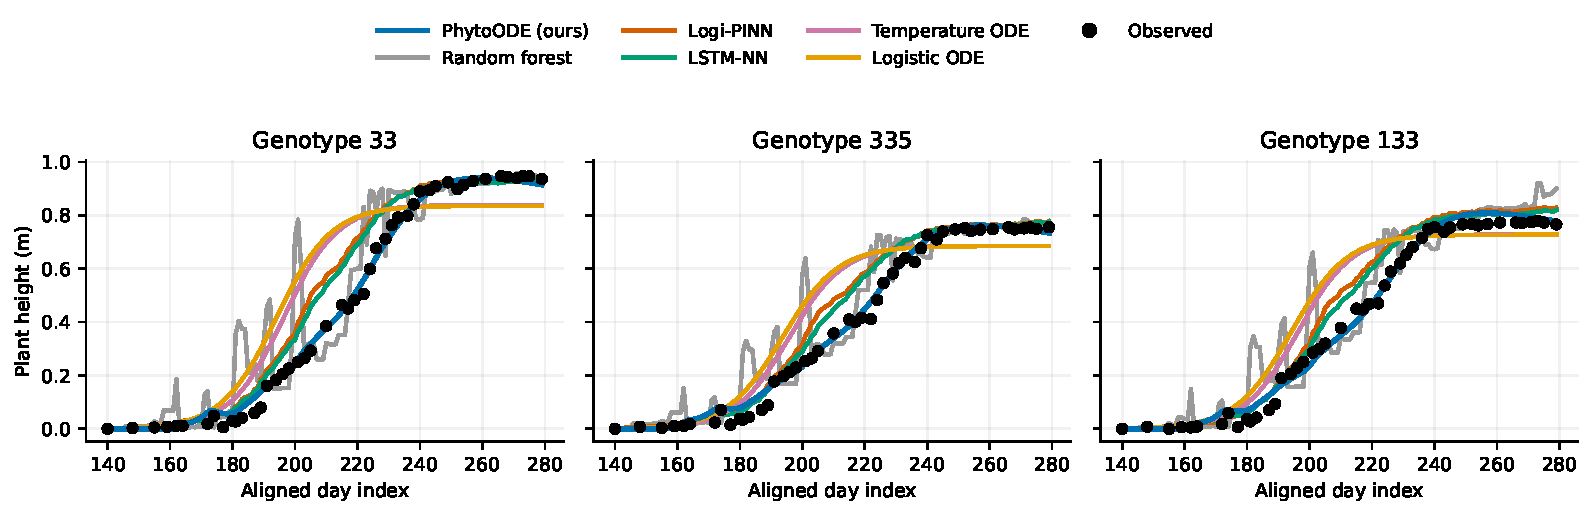
\includegraphics[width=0.96\textwidth]{figures/wheat_test_curves_no_extrapolation.pdf}
\caption{Wheat test observations and predictions in the held-out 2021 season for three genotypes selected with a fixed random seed. Black points are replicate-averaged observations, and colored lines are predictions from the six compared methods using the common legend. Lines for \model{}, RF, LSTM-NN, and Logi-PINN are seed means; Temperature ODE and Logistic ODE are single deterministic fits. Every curve is restricted to the interval between the first and last actual observations.}
\label{fig:wheatcurves}
\end{figure*}

Figure~\ref{fig:wheatcurves} places all six methods on the same trajectories and shows that \model{} captured genotype-dependent onset, rapid elongation, and plateau height while avoiding the irregular RF interpolation and the earlier plateaus of the fixed-form ODEs in these examples. Achieving the lowest test error with only 1,655 parameters, compared with 4,647 before capacity tuning, supports parameter-efficient transfer across field seasons. The displayed curves deliberately end with the data. Consequently, this experiment establishes performance over the measured support in a new year for 19 observed genotypes, not unseen-genotype prediction or forecasting beyond the final phenotyping date.

\subsection{Maize: year-held-out prediction across 402 genotypes}
\label{subsec:maizeresults}

With the retained $(\lambda_{\mathrm{ODE}},\lambda_K)=(0.5,0.5)$ configuration, \model{} achieved the lowest mean test error among the five benchmark families and the no-physics latent ODE control, with RMSE / rRMSE of $56.68\pm4.37$ relative UAV-height units / $18.40\pm1.42\%$ (Table~\ref{tab:maize}). This reduced the pre-tuning test rRMSE from $25.84\pm4.26\%$ by 28.8\% and was 42.6\% lower than the best test result among the five benchmark families, $32.06\pm3.31\%$ from LSTM-NN. RF again fitted the training data most closely but produced the largest test error. LSTM-NN had the lowest 2020 validation error, while \model{} ranked first in 2021; this reversal indicates substantial interannual variation and motivates future evaluation over multiple validation--test year rotations.

\begin{table*}[t]
\centering
\small
\caption{Maize trajectory errors: training on 2018--2019, validation on 2020, and testing on 2021. Each cell reports RMSE in relative UAV-height units / rRMSE (\%). Bold indicates the lowest mean in each split. Stochastic-model values are mean $\pm$ sample standard deviation over seeds 1--3; process ODEs were fitted once. Only PhytoODE received the additional hyperparameter search; its retained coefficient setting and the matched no-physics control are described in Section~\ref{subsec:physicsablationmethods}.}
\label{tab:maize}
\resizebox{\textwidth}{!}{%
\begin{tabular}{lccc}
\toprule
Model & Train RMSE / rRMSE & Validation RMSE / rRMSE & Test RMSE / rRMSE \\
\midrule
Logi-ODE & $47.29\,/\,15.15$ & $124.63\,/\,49.17$ & $128.98\,/\,41.87$ \\
Temp-ODE & $47.35\,/\,15.17$ & $110.12\,/\,43.45$ & $110.29\,/\,35.80$ \\
RF & $\mathbf{7.03\pm0.01\,/\,2.25\pm0.00}$ & $131.78\pm0.95\,/\,51.99\pm0.37$ & $139.61\pm0.31\,/\,45.31\pm0.10$ \\
LSTM-NN & $42.62\pm1.73\,/\,13.66\pm0.55$ & $\mathbf{40.92\pm2.21\,/\,16.15\pm0.87}$ & $98.77\pm10.20\,/\,32.06\pm3.31$ \\
Logi-PINN & $33.18\pm2.07\,/\,10.63\pm0.66$ & $48.14\pm8.37\,/\,19.00\pm3.30$ & $108.71\pm44.42\,/\,35.28\pm14.42$ \\
Latent ODE (no physics) & $43.25\pm5.76\,/\,13.86\pm1.85$ & $60.75\pm10.03\,/\,23.97\pm3.96$ & $67.78\pm13.62\,/\,22.00\pm4.42$ \\
\model{} (ours) & $41.90\pm14.37\,/\,13.43\pm4.61$ & $47.25\pm2.60\,/\,18.64\pm1.03$ & $\mathbf{56.68\pm4.37\,/\,18.40\pm1.42}$ \\
\bottomrule
\end{tabular}%
}
\end{table*}

\begin{figure*}[t]
\centering
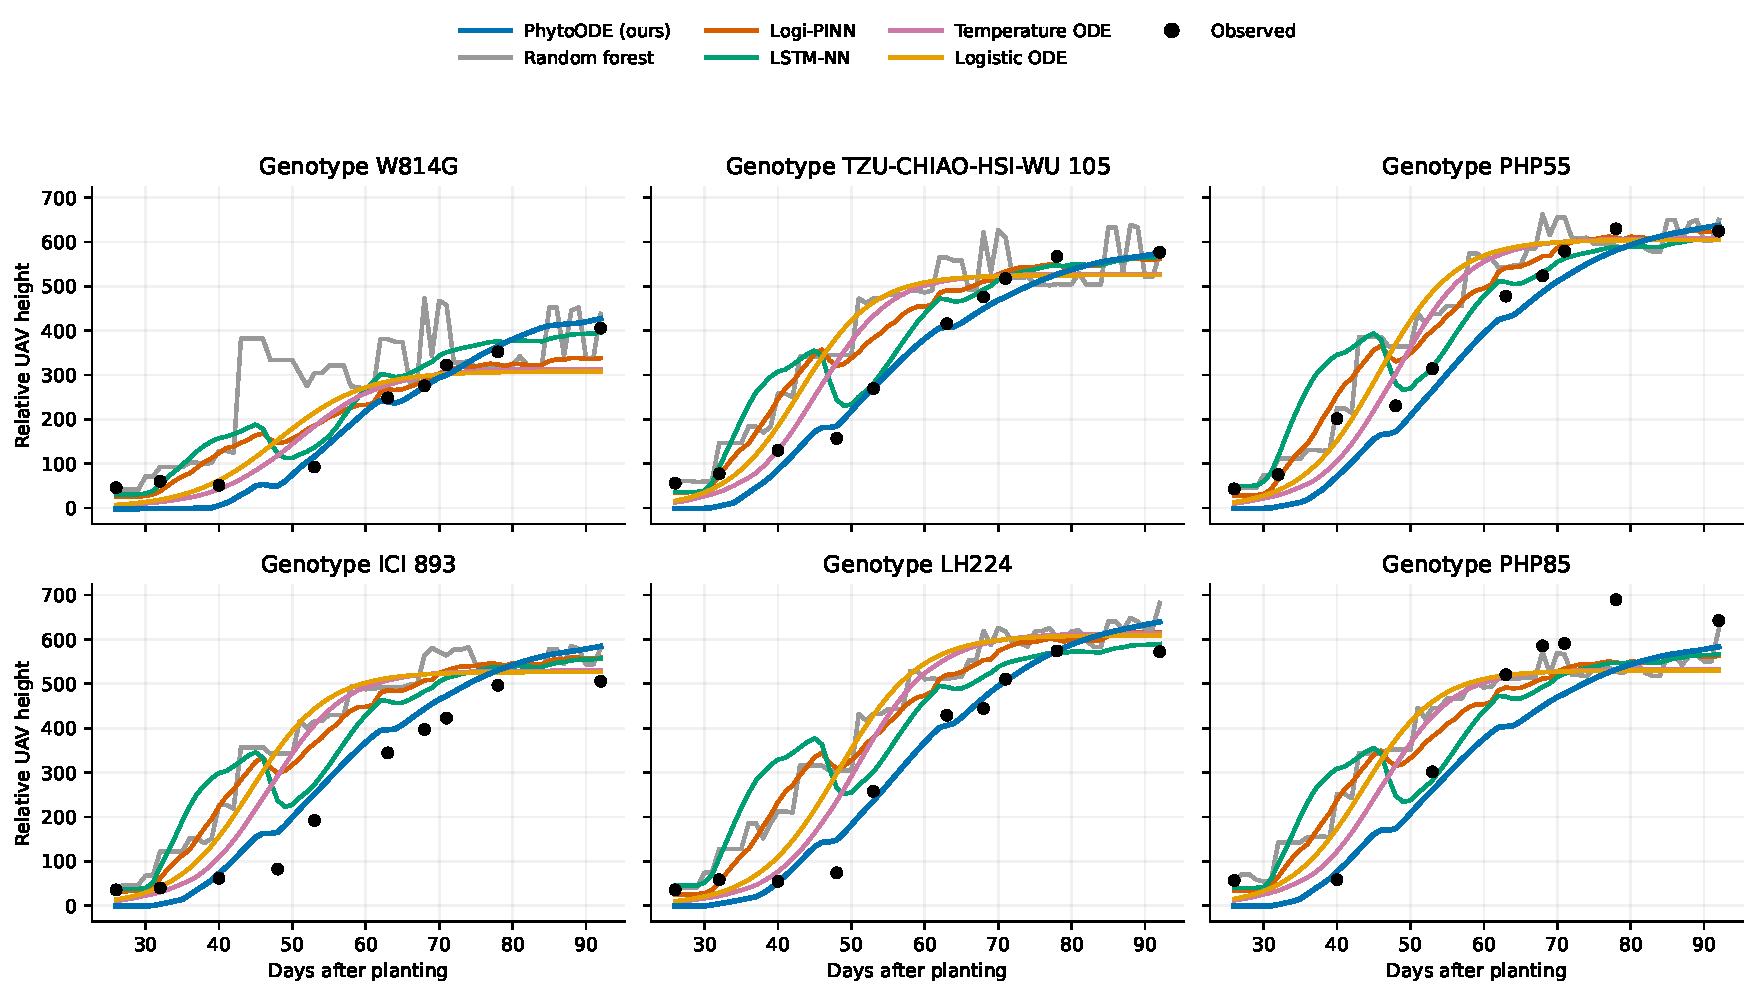
\includegraphics[width=0.98\textwidth]{figures/maize_test_predictions.pdf}
\caption{Maize test observations and predictions in the held-out 2021 season for six genotypes spanning error strata fixed before tuning. Black points are genotype-mean UAV observations, and colored lines are predictions from the six compared methods using the common legend. Lines for \model{}, RF, LSTM-NN, and Logi-PINN are seed means; Temperature ODE and Logistic ODE are single deterministic fits. The \model{} curves use the retained $(\lambda_{\mathrm{ODE}},\lambda_K)=(0.5,0.5)$ configuration. Every curve is restricted to the interval between the first and last observations.}
\label{fig:maizecurves}
\end{figure*}

Figure~\ref{fig:maizecurves} compares PhytoODE and the five benchmark families and shows differences in inferred growth onset and late-season height across contrasting error strata. The 402-genotype evaluation is 21 times larger in genotype count than wheat and approximately 45 times larger than Arabidopsis, providing evidence that a shared latent vector field and learned genotype embeddings can scale to a genetically broad panel without fitting an independent dynamical system to every line. Because the same genotype identities occur in all four seasons, this result concerns environmental transfer across a large observed panel; genotype-held-out evaluation remains necessary before claiming prediction for novel lines.

\subsection{Arabidopsis: external validation with four observations per plant}
\label{subsec:arabresults}

\model{} achieved the lowest mean validation and test errors on the Arabidopsis primary-stem dataset (Table~\ref{tab:arabidopsis}). Its test RMSE / rRMSE was $2.800\pm0.016$~cm / $14.06\pm0.08\%$, compared with $2.878\pm0.010$~cm / $14.45\pm0.05\%$ for RF and $2.993\pm0.066$~cm / $15.03\pm0.33\%$ for the no-physics latent ODE. These correspond to mean test RMSE reductions of 2.7\% and 6.46\%, respectively. This ordering was obtained with only four observed dates per plant, supporting the applicability of the regularized continuous-time model under sparse temporal sampling; three initialization seeds alone do not establish statistical significance.

\begin{table*}[t]
\centering
\small
\caption{Arabidopsis primary inflorescence stem-length errors under the plant-held-out split. Each cell reports RMSE in centimetres / rRMSE (\%). Bold indicates the lowest mean in each split. Stochastic-model values are mean $\pm$ sample standard deviation over seeds 1--3; process ODEs were fitted once. Each validation and test trajectory contains four observed time points.}
\label{tab:arabidopsis}
\resizebox{\textwidth}{!}{%
\begin{tabular}{lccc}
\toprule
Model & Train RMSE / rRMSE & Validation RMSE / rRMSE & Test RMSE / rRMSE \\
\midrule
Logi-ODE & $4.944\,/\,23.50$ & $5.274\,/\,26.19$ & $5.179\,/\,26.00$ \\
Temp-ODE & $3.678\,/\,17.48$ & $4.174\,/\,20.73$ & $4.121\,/\,20.69$ \\
RF & $\mathbf{0.153\pm0.018\,/\,0.73\pm0.08}$ & $3.217\pm0.008\,/\,15.97\pm0.04$ & $2.878\pm0.010\,/\,14.45\pm0.05$ \\
LSTM-NN & $1.701\pm0.122\,/\,8.09\pm0.58$ & $3.343\pm0.103\,/\,16.60\pm0.51$ & $2.951\pm0.064\,/\,14.82\pm0.32$ \\
Logi-PINN & $1.721\pm0.034\,/\,8.18\pm0.16$ & $3.316\pm0.075\,/\,16.47\pm0.37$ & $2.987\pm0.126\,/\,15.00\pm0.63$ \\
Latent ODE (no physics) & $1.188\pm0.028\,/\,5.64\pm0.13$ & $3.278\pm0.047\,/\,16.28\pm0.23$ & $2.993\pm0.066\,/\,15.03\pm0.33$ \\
\model{} (ours) & $1.421\pm0.030\,/\,6.75\pm0.14$ & $\mathbf{3.191\pm0.033\,/\,15.85\pm0.16}$ & $\mathbf{2.800\pm0.016\,/\,14.06\pm0.08}$ \\
\bottomrule
\end{tabular}%
}
\end{table*}

RF attained the smallest training error, while \model{} attained the smallest mean validation and test errors. The no-physics latent ODE also fitted the training curves more closely than \model{} but generalized less accurately to the held-out plants. These results are consistent with a benefit from the combined growth regularizers under sparse observation, while the small advantage over RF should be assessed on additional biological cohorts.

When evaluated separately by temperature regime, \model{} achieved RMSEs of $2.126\pm0.056$~cm under nAT and $3.474\pm0.047$~cm under hAT. Random forest was better under hAT ($3.342\pm0.032$~cm) but worse under nAT ($2.414\pm0.037$~cm). The hAT trajectories begin and terminate earlier and often approach a plateau by 41 DAS, making their timing difficult to infer from four observations. Figure~\ref{fig:arabcurves} illustrates Col-0 predictions under both temperature regimes. All curves between observed points are model-based interpolation, not additional biological observations.

\begin{figure*}[t]
\centering

\includegraphics[width=0.96\textwidth]{figures/arabidopsis_col0_no_extrapolation.pdf}
\caption{Arabidopsis Col-0 test observations and predictions under normal (nAT) and high (hAT) ambient temperature. Black points are means of the two held-out test plants, and colored lines are predictions from the six compared methods using the common legend. Lines for \model{}, RF, LSTM-NN, and Logi-PINN are seed means; Temperature ODE and Logistic ODE are single deterministic fits. Every curve is restricted to the condition-specific observation interval (nAT: 29--49 DAS; hAT: 27--41 DAS).}
\label{fig:arabcurves}
\end{figure*}

Taken together, the Arabidopsis results support resilience to low temporal resolution in a species and organ distinct from the wheat development dataset. However, this evidence is bounded: all nine genotypes and both temperature regimes occur in training, validation, and test splits, and each test curve averages only two plants. The experiment therefore supports cross-species, sparse-trajectory applicability but not genotype or environmental extrapolation.


\subsection{Hypocotyl growth: individual observations under light regimes}
\label{subsec:hypocotylresults}

The author-collected experiment tests environmental-driver substitution and learning from incomplete replicate observations. Temperature was fixed at 23~$^{\circ}$C, while the known illumination schedule supplied the environmental input. All models were trained directly on the 1,052 measured training lengths. Table~\ref{tab:hypocotyl_replicate} reports errors against the 330 validation and 436 test measurements individually, without constructing replicate-mean targets. The same seven observed times and ten genotype--condition combinations occur in each partition.

Validation selected a 1,160-parameter \model{} with latent dimension 8, genotype embedding 4, vector-field width 16 and depth 1, decoder width 16, and encoder width 8. The learning rate was 0.01, weight decay 0.0001, and $(\lambda_{\mathrm{ODE}},\lambda_K)=(0.0161777,0.000813047)$. All neural candidates used 2,000 epochs and validation-selected checkpoints.

\model{} achieved test RMSE / relative RMSE of $0.7788\pm0.0061$~mm / $13.72\pm0.11\%$, compared with $0.7815\pm0.0045$~mm / $13.77\pm0.08\%$ for the independently tuned no-physics latent ODE. The smallest mean test RMSE was attained by LSTM-NN ($0.7741$~mm / $13.64\%$).

\begin{table}[t]
\centering
\small
\caption{Hypocotyl replicate-group holdout: individual-observation RMSE (mm) / relative RMSE (\%). Each measured cell is scored separately. Stochastic models report mean $\pm$ sample SD across three seeds; process ODEs are single fits. Bold marks the smallest unrounded mean in each split. The matched control uses the selected PhytoODE architecture and training settings with both physics coefficients zero.}
\label{tab:hypocotyl_replicate}
\resizebox{\linewidth}{!}{%
\begin{tabular}{lccc}
\toprule
Model & Train & Validation & Test \\
\midrule
PhytoODE & $0.754\pm0.007 / 13.16\pm0.11$ & $0.718\pm0.001 / 12.33\pm0.03$ & $0.779\pm0.006 / 13.72\pm0.11$ \\
Latent ODE (no physics) & $0.755\pm0.002 / 13.19\pm0.03$ & $\mathbf{0.716\pm0.001 / 12.29\pm0.02}$ & $0.782\pm0.005 / 13.77\pm0.08$ \\
Light-PINN & $0.767\pm0.005 / 13.40\pm0.08$ & $0.726\pm0.004 / 12.47\pm0.08$ & $0.793\pm0.005 / 13.97\pm0.08$ \\
LSTM-NN & $0.739\pm0.002 / 12.91\pm0.04$ & $0.719\pm0.006 / 12.35\pm0.10$ & $\mathbf{0.774\pm0.003 / 13.64\pm0.05}$ \\
Random forest & $\mathbf{0.731\pm0.000 / 12.77\pm0.00}$ & $0.728\pm0.000 / 12.51\pm0.01$ & $0.778\pm0.001 / 13.71\pm0.01$ \\
Light-logistic ODE & $0.821 / 14.34$ & $0.802 / 13.77$ & $0.844 / 14.86$ \\
Logistic ODE & $0.807 / 14.10$ & $0.771 / 13.24$ & $0.827 / 14.57$ \\
\midrule
Latent ODE (matched) & $0.751\pm0.005 / 13.12\pm0.09$ & $0.718\pm0.002 / 12.32\pm0.04$ & $0.777\pm0.005 / 13.69\pm0.09$ \\
\bottomrule
\end{tabular}}
\end{table}


The control with the same architecture, optimizer settings, initial weights, schedule, and checkpoint rule, but both physics coefficients zero, obtained $0.7769\pm0.0049$~mm / $13.69\pm0.09\%$. \model{} had 0.24\% higher mean test RMSE than this control. This comparison measures the combined contribution of the derivative and capacity penalties. The independently tuned latent ODE has the same number of screening and confirmation fits as \model{}; its configuration is selected separately by validation.

\begin{figure}[!htbp]
\centering
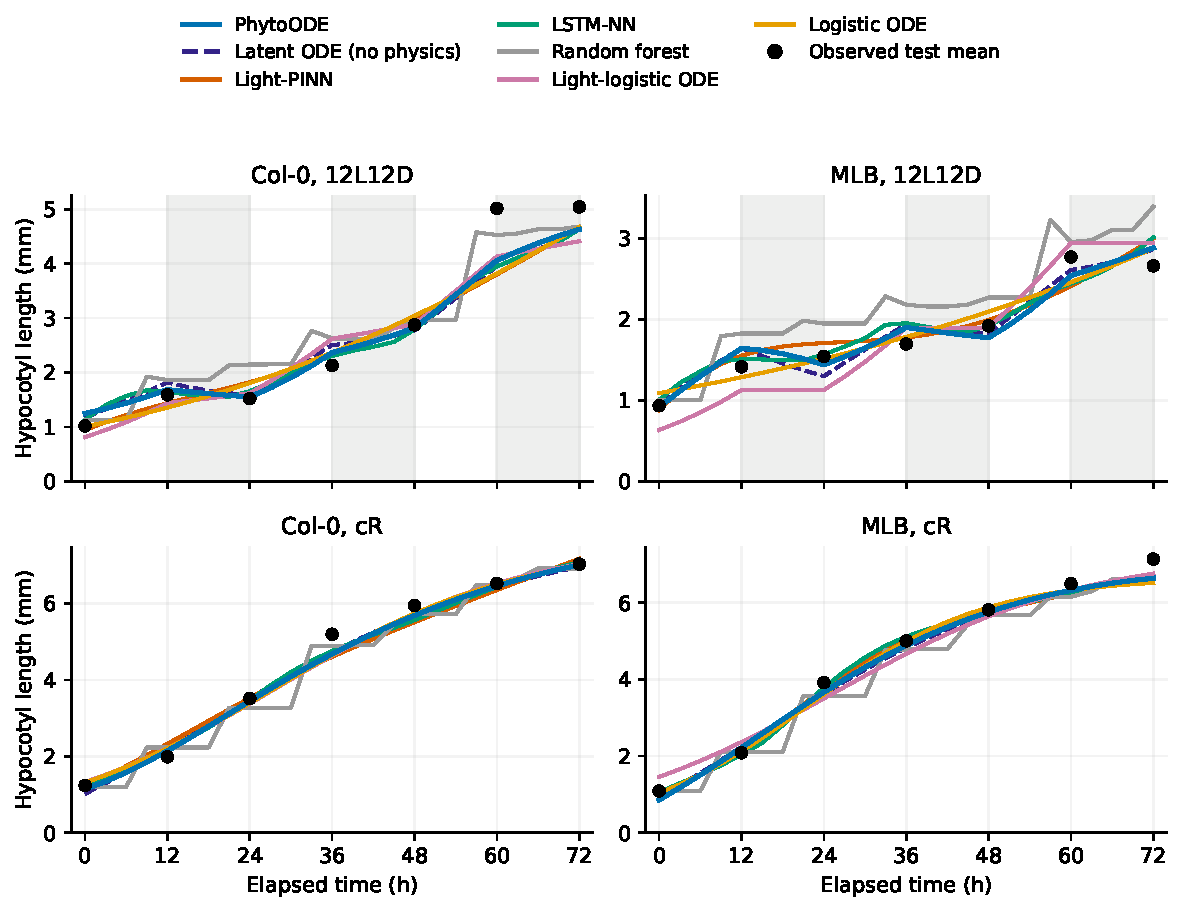
\includegraphics[width=0.96\linewidth]{figures/hypocotyl_light_replicates.pdf}
\caption{Hypocotyl predictions for Col-0 and MLB under 12L12D and continuous red light (cR). Every black point is one held-out measured length; observations are not averaged. Small horizontal offsets separate overlapping points and do not change their recorded times. Colored curves show the mean prediction across three training seeds, except for the single-fit process ODEs. Gray shading indicates darkness in 12L12D. All seven times are represented in training and validation using separate replicate groups. Each genotype--condition curve is fitted to individual measurements, without inferring longitudinal plant identities. The matched loss-removal control is reported in Table~\ref{tab:hypocotyl_replicate}; all five genotypes are shown in the accompanying full-panel figure.}
\label{fig:hypocotyllight}
\end{figure}

This experiment demonstrates a shared growth-prediction framework across species, organs, scales, and environmental drivers. Its seven measurement times remain sparse relative to the continuous latent dynamics, and unequal replicate counts and missing cells are handled by evaluating residuals only where measurements exist. Observation-level scoring retains the variation among measured plants. Since individual covariates are unavailable, plants with the same genotype, lighting regime, and observation time receive the same predicted length; the experiment does not establish individualized trajectory recovery.

The original workbook, cell-level provenance, extraction checks, and fixed partitions form a reproducible author-collected dataset package. Both light regimes and all five genotypes are represented during training. A single temperature cannot identify temperature dependence, and the unrecorded 12L12D spectrum prevents separation of spectral and photoperiod effects. The phase-specific logistic rates provide a compact reference, while 12-h sampling and unknown plant identities and batch structure limit inference about circadian timing and independent-cohort generalization.

Halving the integration step from 3 to 1.5~h while preserving the encoder inputs changed \model{} predictions by at most 0.000010~mm across the three seeds.

\FloatBarrier


\subsection{Contribution of the physics regularizers}
\label{subsec:physicsablationresults}

Relative to the matched latent ODE with both physics coefficients set to zero, the adopted PhytoODE configurations reduced mean test RMSE by 1.91\% for wheat, 16.37\% for maize, and 6.46\% for Arabidopsis (Tables~\ref{tab:wheat}--\ref{tab:arabidopsis}). This comparison concerns the combined derivative-residual and carrying-capacity penalties. It does not isolate the contribution of the derivative residual alone. In particular, the maize K-only model achieved a slightly lower mean test RMSE / rRMSE of $55.83\pm6.15$ / $18.12\pm2.00\%$ than the adopted full model, although its validation RMSE was higher (48.143 versus 47.247). Therefore, these results support a benefit of the adopted physics-regularized configuration over the both-zero control under the recorded training settings, but not a universal test-error benefit from adding the derivative residual to K regularization. The no-physics control was not separately retuned, and the reused test sets limit independent confirmation.

\section{Conclusion}
\label{sec:conclusion}

We introduced \model{}, a genotype- and environment-conditioned latent neural ODE model for predicting plant growth trajectories. The three temperature-conditioned benchmarks and the additional light-conditioned hypocotyl experiment test distinct observation settings. It achieved lower mean test RMSE than the five benchmark families and the matched no-physics latent ODE in wheat, maize, and Arabidopsis, with rRMSEs of $10.24\pm0.22\%$, $18.40\pm1.42\%$, and $14.06\pm0.08\%$, respectively. The wheat result combines year-held-out accuracy with a compact 1,655-parameter model. The maize result extends the same model family to 402 genotypes and 3,072 field-plot trajectories, showing that genotype-conditioned latent dynamics can scale to a substantially broader observed panel. The Arabidopsis result remains competitive with RF despite only four measurements per plant and transfers the formulation to a different species, organ, and growth scale. Together, these results provide complementary evidence for parameter-efficient field-season transfer, high-cardinality genotype conditioning, and resilience to sparse temporal observation.

The hypocotyl experiment extends the formulation to explicit illumination at fixed temperature and direct fitting to incomplete individual observations. On 436 held-out measured lengths, its test relative RMSE was $13.72\%$, compared with $13.77\%$ for the independently tuned no-physics latent ODE and $13.69\%$ for the matched control. All seven times are represented in each partition, and missing phenotype cells contribute no data residual. The accompanying data package makes extraction and partitioning inspectable. Further biological evaluation requires independently documented cohorts and more complete light metadata.

Four limitations define the next experiments. First, capacity and hyperparameters were tuned on a single validation year for wheat and maize, and the subsequent coefficient study reused previously inspected test sets. The retained maize setting also differs from the later validation optimum. Fixed configurations and independently tuned controls should therefore be evaluated over additional validation--test year rotations and independent cohorts. Second, both year-held-out experiments contain the same genotype identities across years, so the 402-genotype maize result demonstrates scale across observed lines rather than prediction of unseen genotypes. Third, the Arabidopsis split holds out plants rather than genotypes or temperature regimes and averages only two test plants per genotype--temperature combination. Independent cohorts, genotype-held-out validation, and intermediate or fluctuating temperature treatments would provide stronger biological tests. Fourth, the present evaluation and figures are restricted to measured temporal support and do not establish accuracy beyond the last phenotyping date. A causal forecasting variant should restrict the environmental encoder to temperatures available up to the forecast origin and evaluate explicitly defined extrapolation horizons.

\section*{Data and code availability}
The three published datasets are identified in Sections~\ref{subsec:wheatdata}--\ref{subsec:arabdata}. For the new hypocotyl dataset, we have prepared the original workbook, cell-resolved measurements, metadata, frozen partitions, extraction checks, and analysis code for release alongside the model configurations, checkpoints, and prediction arrays. A verified public repository URL or permanent dataset identifier and a data-reuse license must be added before publication; public availability is not asserted in this draft.

\section*{Declaration of competing interest}
The authors declare that they have no known competing financial interests or personal relationships that could have appeared to influence the work reported in this paper.

\section*{Acknowledgements}
Hwijae Son was supported by the Basic Science Research Program through the National Research Foundation of Korea (NRF), funded by the Ministry of Education (RS-2026-25491905 and RS-2026-25506577).

\bibliographystyle{elsarticle-harv}
\bibliography{references}

\end{document}
